% !TEX encoding = cp1250
\chapter{�wiczenie laboratoryjne}
Mo�na napisa� o tym, �e realizowane w MATLABie i jakie oznaczenia maj� jakie rzeczy (W1 ma index 1,  G1 jaki index i T1 jaki index)

\section{Przygotowanie do wykonania �wiczenia}
Przed rozpocz�ciem pomiar�w sprawdzono mo�liwo�� sterowania i~pomiaru w~komunikacji ze stanowiskiem. Punkt pracy grza�ki $G1$ dla zespo�u obliczony zosta� wg. wzoru \ref{w_G1}:
\begin{equation}
	G1 = 25 + Z\%5\
\label{w_G1}
\end{equation}
gdzie Z~to numer zespo�u, zatem dla naszego zespo�u Z02 punkt pracy wynosi:
\begin{equation}
	G1 = 25 + 2\%5 = 27
\end{equation}
Nast�pnie okre�lono warto�� pomiaru temperatury T1 dla obliczonego punktu pracy. W~tym celu moc wentylatora W1 ustawiono na 50\%, a moc grza�ki G1 na 27\%,  za pomoc� funkcji
\texttt{sendControls([1,5], [50,27])}.
Warto�� pomiaru temperatury odczytano korzystaj�c z~funkcji 
\texttt{readMeasurements(1)}.
Temperatura T1 ustabilizowa�a si� na warto�ci \textbf{32.25\degree C}

 
\section{Wyznaczenie odpowiedzi skokowych procesu}
Zarejestrowano przebieg temperatury T1 dla trzech r�nych zmian sygna�u steruj�cego G1 rozpoczynaj�c z~punktu pracy (27\%) do 10\%, 35\% i~50\%.
Otrzymane przebiegi zmian przedstawiono na Rys. \ref{rys_przebiegi_T1}. 

\textcolor{red}{
	Czy w�a�ciwo�ci statyczne obiektu mo�na okre�li� jako (w przybli�eniu) liniowe? Je�li tak wyznaczy� wzmocnienie statyczne procesu?
}

\newpage
\begin{figure}[H]
	\centering
	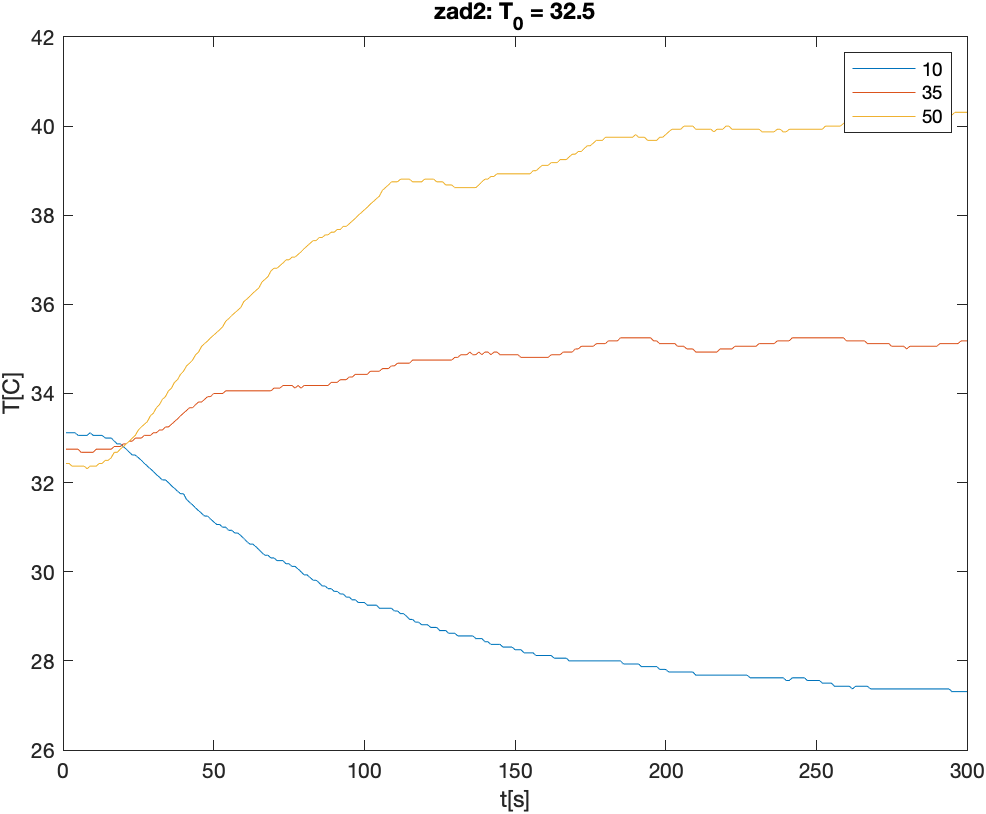
\includegraphics[scale=0.35]{png/lab1_zad2.png}
	\caption{Odpowiedzi skokowe procesu}
	\label{rys_przebiegi_T1}
\end{figure}

\section{Algorytm DMC}

